% !TeX program = xelatex
% 第三章 3.3：接在 03_02_augmented_prediction.tex 之後。
% 需要 amsmath、amssymb；章節與公式由 LaTeX 自動編號。
% 新增引用鍵：goldfarb1983dual、stellato2020osqp。

% ==================================================
% 3.3 全身預測控制之目標函數與限制條件
% ==================================================
\section{全身預測控制之目標函數與限制條件}
\label{sec:wholebody_objective_constraints}

本節以前述增廣預測模型為基礎，建立底盤與手臂共同求解的有限時域控制問題。目標函數同時考量底盤追蹤、末端位姿追蹤及命令平順性，並納入實際關節位置、位置設定點與底盤輪級運動限制。透過共同的末端追蹤目標，控制器可在可用運動範圍內分配底盤與手臂的運動，使導航參考與操作需求共同影響控制輸出。本節先建立基本控制問題，障礙與受約束操作之附加條件於後續各節說明。

% ==================================================
% 3.3.1 底盤與末端位姿追蹤目標
% ==================================================
\subsection{底盤與末端位姿追蹤目標}
\label{subsec:wholebody_tracking_objective}

沿用前節的預測索引，令 $e_{B,i|k}$ 為底盤幾何追蹤誤差。以 $\|x\|_Q^2=x^{\top}Qx$ 表示加權平方範數，底盤追蹤成本定義為
\begin{equation}
    J_B=
    \sum_{i=1}^{N-1}\|e_{B,i|k}\|_{Q_B}^{2}
    +\|e_{B,N|k}\|_{Q_{B,f}}^{2},
    \label{eq:ch3_base_tracking_cost}
\end{equation}
其中 $Q_B$ 為階段權重，$Q_{B,f}$ 為終端權重，分別調整預測時域內及末端時刻的追蹤需求。

令 $p_{E,i|k}$ 與 $R_{E,i|k}$ 為預測末端在世界座標中的位置及姿態，$p_{E,i|k}^{d}$ 與 $R_{E,i|k}^{d}$ 為對應目標。定義末端位姿殘差為
\begin{equation}
    r_{E,i|k}=
    \begin{bmatrix}
        p_{E,i|k}^{d}-p_{E,i|k} \\
        R_{E,i|k}
        \left[\log\!\left(R_{E,i|k}^{\top}R_{E,i|k}^{d}\right)\right]^{\vee}
    \end{bmatrix}
    \in\mathbb{R}^{6}.
    \label{eq:ch3_tcp_pose_residual}
\end{equation}
姿態殘差由相對旋轉的對數映射取得，並轉換至世界座標，使其與前節的末端幾何雅可比採用相同座標表示。末端追蹤成本為
\begin{equation}
    J_E=\sum_{i=1}^{N}\|r_{E,i|k}\|_{W_E}^{2},
    \qquad
    W_E=\operatorname{diag}(W_p,W_R),
    \label{eq:ch3_tcp_tracking_cost}
\end{equation}
其中 $W_p$ 與 $W_R$ 分別為位置及姿態權重。底盤與手臂均會改變世界座標中的末端位姿，因此，此成本可形成兩者共同承擔操作目標的機制。本節先以世界座標目標說明；持物運送等採用底盤相對目標的情況，於任務參考與操作設計中另行定義。

為限制控制輸入大小並抑制相鄰命令的急遽變化，另建立
\begin{equation}
    \begin{aligned}
        J_U
        &=\sum_{i=0}^{N-1}
          \left(
              \|\delta\xi_{i|k}\|_{R_{\xi}}^{2}
              +\|u_{a,i|k}\|_{R_a}^{2}
          \right), \\
        J_{\Delta}
        &=\sum_{i=0}^{N-1}
          \left(
              \|\Delta\xi_{B,i|k}\|_{S_{\xi}}^{2}
              +\|\Delta u_{a,i|k}\|_{S_a}^{2}
          \right),
    \end{aligned}
    \label{eq:ch3_input_smoothness_cost}
\end{equation}
其中底盤速度命令為 $\xi_{B,i|k}=\xi_{r,k+i}+\delta\xi_{i|k}$，命令差分定義為 $\Delta\xi_{B,i|k}=\xi_{B,i|k}-\xi_{B,i-1|k}$ 及 $\Delta u_{a,i|k}=u_{a,i|k}-u_{a,i-1|k}$。第一步差分以前一筆實際生效命令為基準；若預測起點經延遲補償前推，則使用該起點之前的生效命令。底盤平順性成本計算的是完整速度命令之差，須包含參考速度的變化。

基本目標函數為 $J=J_B+J_E+J_U+J_{\Delta}$。各追蹤與平順性權重選為半正定矩陣，輸入權重則提供控制量的正則化。位置、角度及命令具有不同單位，其權重依容許尺度設定，實驗使用之數值於第四章說明。

% ==================================================
% 3.3.2 關節、命令變化與輪級運動限制
% ==================================================
\subsection{關節、命令變化與輪級運動限制}
\label{subsec:joint_command_wheel_constraints}

手臂位置設定點與實際關節位置具有不同的追蹤動態，因此，兩者皆需納入位置限制。令 $q_{\min}$、$q_{\max}$ 為關節位置界限，$\mu\in\mathbb{R}_{\geq0}^{6}$ 為限位餘量，則對 $i=1,\ldots,N$，施加
\begin{equation}
    \begin{aligned}
        q_{\min}+\mu
        &\leq q_{a,i|k}\leq q_{\max}-\mu, \\
        q_{\min}+\mu
        &\leq s_{a,i|k}\leq q_{\max}-\mu.
    \end{aligned}
    \label{eq:ch3_joint_setpoint_limits}
\end{equation}
上述不等式均依元素成立。當追蹤模型包含偏置或設定點與實際位置尚未一致時，兩組限制無法直接互相取代。

底盤與手臂命令另需滿足
\begin{equation}
    \begin{aligned}
        \xi_{\min}
        &\leq\xi_{B,i|k}\leq\xi_{\max}, \\
        -\bar{a}_B\Delta t
        &\leq\Delta\xi_{B,i|k}\leq\bar{a}_B\Delta t, \\
        -\bar{v}_s
        &\leq u_{a,i|k}\leq\bar{v}_s, \\
        -\bar{a}_s\Delta t
        &\leq\Delta u_{a,i|k}\leq\bar{a}_s\Delta t,
    \end{aligned}
    \label{eq:ch3_command_rate_limits}
\end{equation}
其中 $i=0,\ldots,N-1$，$\bar{a}_B$ 為底盤速度命令的變化率上限，$\bar{v}_s$ 與 $\bar{a}_s$ 分別為手臂設定點變化率及其變化率的上限。手臂限制施加於命令介面，實際關節運動則由前節的追蹤模型預測，兩者須分別解讀。

對四輪全向底盤，僅限制各軸速度，仍不足以描述平移與旋轉同時發生時的輪速需求。依本研究輪系之輪序及正方向，輪速命令可寫為
\begin{equation}
    \omega_{w,i|k}
    =\frac{1}{r_w}W\xi_{B,i|k},
    \qquad
    W=
    \begin{bmatrix}
        0 & 1 & L \\
        -1 & 0 & L \\
        0 & -1 & L \\
        1 & 0 & L
    \end{bmatrix},
    \label{eq:ch3_wheel_command_mapping}
\end{equation}
其中 $r_w$ 為輪半徑，$L$ 為底盤輪系的幾何參數，$\omega_{w,i|k}\in\mathbb{R}^{4}$ 為四輪轉速命令。輪級限制為
\begin{equation}
    \begin{aligned}
        -\bar{\omega}_w
        &\leq\omega_{w,i|k}\leq\bar{\omega}_w, \\
        -\bar{\alpha}_w\Delta t
        &\leq\omega_{w,i|k}-\omega_{w,i-1|k}
          \leq\bar{\alpha}_w\Delta t,
    \end{aligned}
    \label{eq:ch3_wheel_speed_acceleration_limits}
\end{equation}
其中 $\bar{\omega}_w$ 與 $\bar{\alpha}_w$ 分別為輪速及輪速命令變化率上限。將此限制直接納入最佳化問題，可使底盤平移與旋轉共同使用輪系可用範圍；此處描述的是命令可行性，實際輪速追蹤與運動誤差仍由實驗評估。

% ==================================================
% 3.3.2 十字全向輪之速度可行域
% ==================================================
當四輪採相同角速度上限時，式\eqref{eq:ch3_wheel_command_mapping}可整理為
\begin{equation}
    |v_x|+L|\omega|\leq r_w\bar\omega_w,
    \qquad
    |v_y|+L|\omega|\leq r_w\bar\omega_w.
    \label{eq:ch3_omni_velocity_feasible_region}
\end{equation}
因此，固定旋轉速度下的平移可行域為軸向方框，其邊界隨 $|\omega|$ 增加而縮小；在 $v_y=0$ 的 $v_x$--$\omega$ 剖面則呈菱形，如\cref{fig:ch3_omni_velocity_feasible_set}所示。以 $r_w=0.05$ m、$L=0.245$ m 與 $\bar\omega_w=5.55$ rad/s 為例，獨立速度框內的 $v_x=0.24$ m/s、$\omega=0.8$ rad/s 需要的輪緣速度達 $0.436$ m/s，超過 $0.2775$ m/s 上限。圖中使用未內縮之幾何界限，實驗中的控制餘裕及輪加速度限制另行列示。

\begin{figure}[htbp]
    \centering
    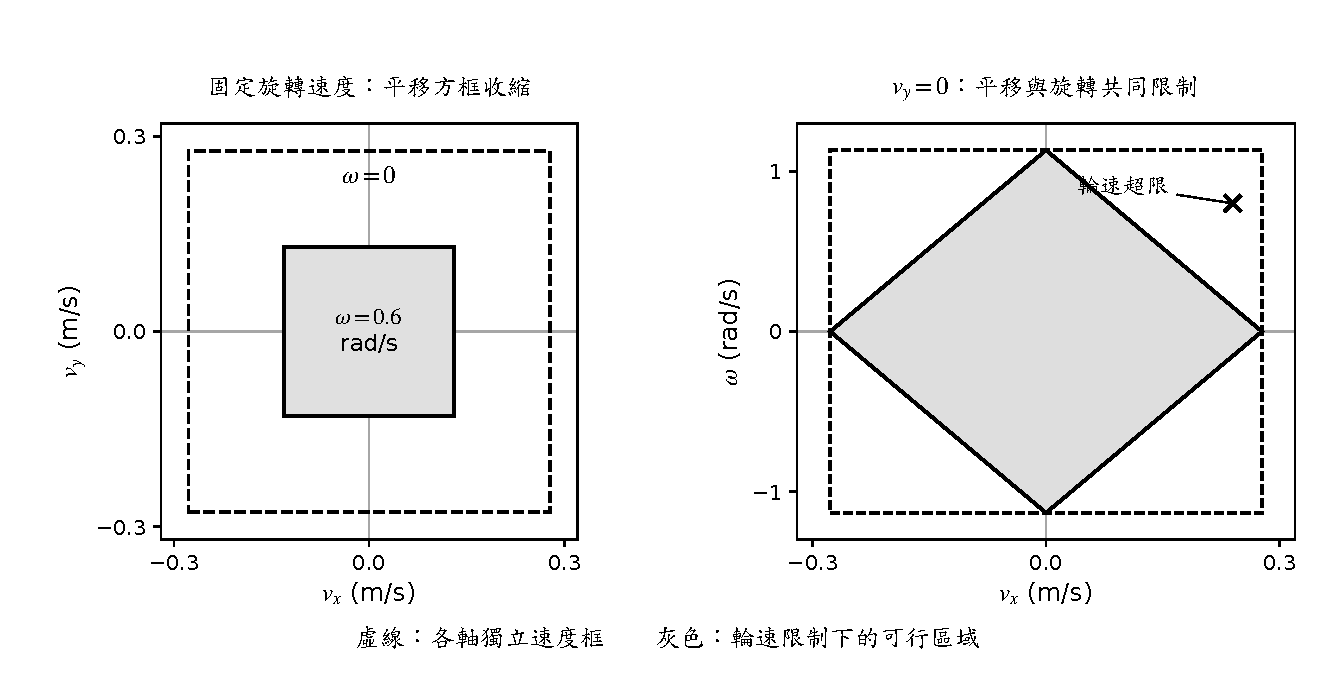
\includegraphics[width=0.98\textwidth]{figsrc/ch03/omni_wheel_velocity_feasible_set.pdf}
    \caption{四輪十字配置之速度可行域：(a) 固定旋轉速度下的 $v_x$--$v_y$ 平移可行域；(b) $v_y=0$ 時的 $v_x$--$\omega$ 剖面。虛線表示各軸獨立速度框，灰色表示輪速限制下的可行區域。}
    \label{fig:ch3_omni_velocity_feasible_set}
\end{figure}

% ==================================================
% 3.3.3 最佳化問題建構與數值求解
% ==================================================
\subsection{最佳化問題建構與數值求解}
\label{subsec:wholebody_qp_formulation}

由式\eqref{eq:ch3_condensed_augmented_prediction}，預測狀態為控制序列 $\mathbf{U}_k$ 的仿射函數。由於末端正向運動學具有非線性，先由給定的控制序列 $\bar{\mathbf{U}}_k$ 計算各步的預測狀態，再於這些狀態建立局部近似。

令 $\Gamma_{i,k}$ 為預測矩陣 $\Gamma_k$ 中對應第 $i$ 步狀態的列區塊，$C_i$ 為底盤幾何誤差至平面位姿座標 $[x_B,y_B,\theta_B]^{\top}$ 的局部微分。以 $J_{\chi,B,i}$ 與 $J_{\chi,A,i}$ 表示前節廣義座標雅可比的底盤及手臂區塊，則末端幾何位移對增廣狀態的局部映射為
\begin{equation}
    \mathcal{J}_{E,i}=
    \begin{bmatrix}
        J_{\chi,B,i}C_i & J_{\chi,A,i} & \mathbf{0}_{6\times6}
    \end{bmatrix}.
    \label{eq:ch3_tcp_augmented_geometric_jacobian}
\end{equation}
各矩陣均於上述預測狀態計算。設定點不直接改變當前末端位姿，其作用經由 $\Gamma_{i,k}$ 中的關節追蹤預測傳遞。

當構型變化與末端姿態誤差均較小時，姿態項採小誤差近似，末端殘差可整理為
\begin{equation}
    \begin{aligned}
        r_{E,i|k}
        &\approx\bar{r}_{E,i|k}
          -L_{i,k}(\mathbf{U}_k-\bar{\mathbf{U}}_k) \\
        &=r_{0,i|k}-L_{i,k}\mathbf{U}_k, \\
        L_{i,k}
        &=\mathcal{J}_{E,i}\Gamma_{i,k}, \\
        r_{0,i|k}
        &=\bar{r}_{E,i|k}+L_{i,k}\bar{\mathbf{U}}_k.
    \end{aligned}
    \label{eq:ch3_tcp_affine_residual}
\end{equation}
其中 $\bar{r}_{E,i|k}$ 為使用 $\bar{\mathbf{U}}_k$ 計算的末端殘差。底盤與手臂的控制分量共同出現在 $L_{i,k}$ 中，故末端追蹤成本可產生底盤與手臂之間的交叉項，使兩者在同一問題中協調運動。

堆疊各步的底盤誤差、末端殘差與完整命令差分，可分別寫成
\begin{equation}
    \begin{aligned}
        \mathbf{E}_{B,k}
        &=M_{B,k}\mathbf{U}_k+c_{B,k}, \\
        \mathbf{r}_{E,k}
        &\approx\mathbf{r}_{0,k}-\mathcal{L}_k\mathbf{U}_k, \\
        \Delta\mathbf{V}_k
        &=D\mathbf{U}_k+c_{\Delta,k}.
    \end{aligned}
    \label{eq:ch3_stacked_objective_maps}
\end{equation}
其中 $M_{B,k}$ 與 $c_{B,k}$ 由增廣預測的底盤列取得，$\mathcal{L}_k$ 與 $\mathbf{r}_{0,k}$ 由式\eqref{eq:ch3_tcp_affine_residual}堆疊而成。$D$ 為相鄰控制輸入的一階差分矩陣，$c_{\Delta,k}$ 則收集參考速度變化及前一筆生效命令造成的常數項。$\Delta\mathbf{V}_k$ 的各步區塊為 $[\Delta\xi_{B,i|k}^{\top},\Delta u_{a,i|k}^{\top}]^{\top}$。

以 $\bar{Q}_B$、$\bar{W}_E$、$\bar{R}$ 與 $\bar{S}$ 表示各預測步權重的分塊對角矩陣，其中 $\bar{Q}_B$ 的最後一塊為 $Q_{B,f}$，$\bar{R}$ 與 $\bar{S}$ 的各步區塊分別為 $\operatorname{diag}(R_{\xi},R_a)$ 與 $\operatorname{diag}(S_{\xi},S_a)$。代入目標函數後，可得二次規劃（Quadratic Programming, QP）問題
\begin{equation}
    \begin{aligned}
        \underset{\mathbf{U}_k}{\operatorname{minimize}}\quad
        &\frac{1}{2}\mathbf{U}_k^{\top}H_k\mathbf{U}_k
          +g_k^{\top}\mathbf{U}_k \\
        \operatorname{subject\ to}\quad
        &\ell_k\leq A_{\mathrm{QP},k}\mathbf{U}_k\leq h_k,
    \end{aligned}
    \label{eq:ch3_wholebody_qp}
\end{equation}
其中，省略與決策變數無關的常數項後，成本矩陣與向量為
\begin{equation}
    \begin{aligned}
        H_k=2\big(&M_{B,k}^{\top}\bar{Q}_B M_{B,k}
             +\mathcal{L}_k^{\top}\bar{W}_E\mathcal{L}_k \\
             &+\bar{R}+D^{\top}\bar{S}D\big), \\
        g_k=2\big(&M_{B,k}^{\top}\bar{Q}_B c_{B,k}
             -\mathcal{L}_k^{\top}\bar{W}_E\mathbf{r}_{0,k} \\
             &+D^{\top}\bar{S}c_{\Delta,k}\big).
    \end{aligned}
    \label{eq:ch3_wholebody_qp_cost_matrices}
\end{equation}
限制矩陣及上下界由前述命令、位置與輪級限制代入仿射預測後建立。當線性化矩陣固定且權重為半正定時，形成凸二次規劃；若輸入權重為正定，則 $H_k$ 為正定，在限制集合非空時具有唯一最小解。此凸性是固定局部近似下的性質，末端運動學仍需隨狀態更新。

本研究的全身耦合問題採用 Goldfarb 與 Idnani\cite{goldfarb1983dual}之對偶作用集法進行數值求解；未取得通過驗證的解時，再以 Stellato 等人\cite{stellato2020osqp}提出之 OSQP 求解相同問題。作用集法所得解以原始問題檢查可行性與 Karush--Kuhn--Tucker（KKT）條件。接受全身控制解前，另檢查命令有限值、預測關節與設定點之限制殘差，以及輸出命令與求解序列的一致性。未通過接受條件時，交由既定的保持或減速機制處理，相關流程於執行動態補償與控制實現一節說明。

% ==================================================
% 3.3.3 底盤與手臂於同一全身控制問題中共同求解
% ==================================================
共同求解的輸入與輸出關係如\cref{fig:ch3_joint_optimization}所示。導航參考與末端操作目標共同作用於同一控制序列，配合增廣模型及限制條件，同時決定底盤速度命令與手臂設定點變化率。

\begin{figure}[htbp]
    \centering
    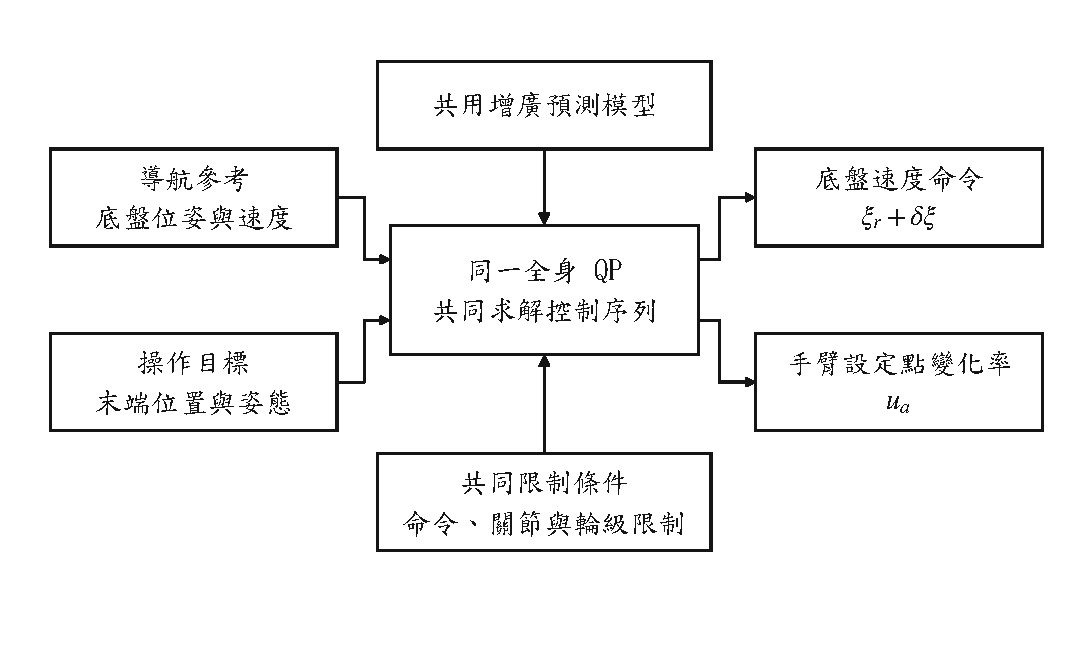
\includegraphics[width=0.98\textwidth]{figsrc/ch03/joint_optimization.pdf}
    \caption{底盤與手臂於同一全身控制問題中共同求解}
    \label{fig:ch3_joint_optimization}
\end{figure}

% ==================================================
% 3.3.4 滾動時域控制原則
% ==================================================
\subsection{滾動時域控制原則}
\label{subsec:wholebody_receding_horizon}

控制器於每個控制週期取得新的機器人狀態與任務參考，依序更新增廣預測、末端局部近似及限制條件，再求解式\eqref{eq:ch3_wholebody_qp}。取得控制序列 $\mathbf{U}_k^{*}$ 後，僅執行首段控制輸入，對應的底盤速度及手臂設定點變化率為
\begin{equation}
    \xi_{B,k}^{\mathrm{cmd}}
    =\xi_{r,k}+\delta\xi_{0|k}^{*},
    \qquad
    u_{a,k}^{\mathrm{cmd}}=u_{a,0|k}^{*}.
    \label{eq:ch3_receding_horizon_command}
\end{equation}
底盤速度送入其執行介面，手臂命令則由執行端依物理步長積分為位置設定點。下一控制週期重新取得實際狀態及設定點後，再進行預測與求解，使追蹤誤差與新觀測能持續影響後續動作。

上述方法以同一有限時域問題協調底盤與手臂，並以命令及狀態限制約束可用運動。後續將加入障礙運動預測與避障條件，進一步說明環境資訊如何轉換為控制問題中的限制。
